\hypertarget{Cext}{\subsection{Secciones transversales}}

En las secciones anteriores se consideró al sistema integrado por una partícula y por una distribución de cargas localizadas en un volumen finito, sometidas a un campo eléctrico homogéneo y a uno armónico, respectivamente. En esta sección, se introducen las denominadas secciones transversales de extinción, absorción y esparcimiento, las cuales son cantidades macroscópicas medibles que proporcionan información sobre el sistema \cite{Bohren}. Para esto, se considera a la partícula embebida en un medio no absorbente e iluminada por una onda plana armónica en el tiempo. Teniendo en cuenta lo anterior, la energía $W_{abs}$, transportada por los campos electromagnéticos y que es absorbida por la partícula, se calcula al integrar el promedio temporal del vector de Poynting \footnote{El promedio temporal del vector de Poynting es $\langle\Vec{S}\rangle_t = (1/\tau)\int_t^{t+\tau}\Vec{S}(t')dt'$, y para campos electromagnéticos del tipo ondas planas es $\langle\Vec{S}\rangle_t = (1/2) \text{Re}[\Vec{E} \times (\Vec{B}/\mu)^{*}]$, donde $*$ corresponde a la operación complejo conjugado \cite{Bohren}. } $\langle\Vec{S}\rangle_t$  sobre una superficie cerrada $A$, que por simplificidad puede considerarse una esfera de radio $r$ mayor al de la partícula (Fig. \ref{WA}), es decir, 
\begin{equation*}
	W_{abs}=-\int_A \langle\Vec{S}\rangle_t\cdot\hat{e}_r \text{ dA},
	\label{flujopoynting}
\end{equation*}
\begin{figure}[h!]
	\centering
	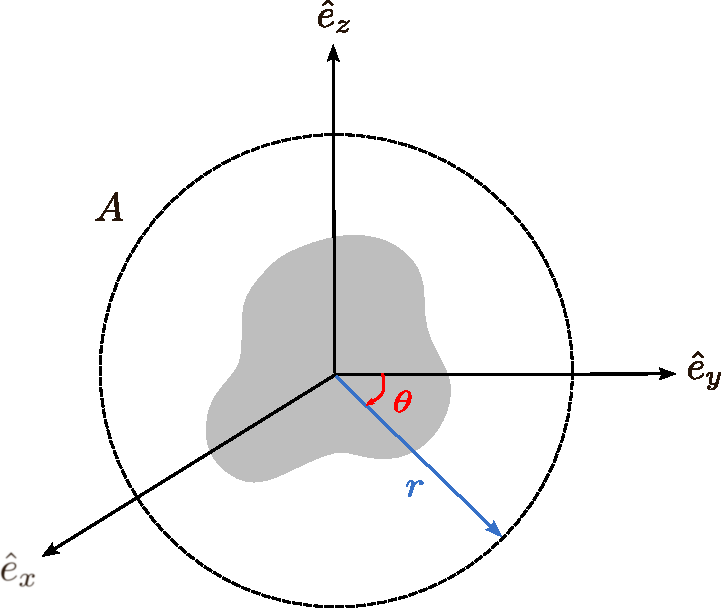
\includegraphics[width=6cm]{../../Figuras/WA.pdf}
	\caption{Esquema de la esfera imaginaria  de radio $r$ y superficie $A$ centrada en el origen y en la partícula de interés.}
	\label{WA}
\end{figure}
donde debido a que $\langle\Vec{S}\rangle_t$ y $\hat{e}_r$ están orientados en la misma dirección, el signo negativo convierte a $W_{abs}$ en una cantidad positiva, de lo contrario, significaría que se genera energía dentro de la esfera \cite{Bohren}. \\

 En este trabajo, el vector de Poynting total se descompone en tres términos \cite{Bohren}
 \begin{equation}
 \langle\Vec{S^i}\rangle_t=  \frac{1}{2}\:\mbox{Re}\{\Vec{E}_i\times\Vec{H}_i^*\}  ,\hspace{0.5cm} \langle\Vec{S^s}\rangle_t=  \frac{1}{2}\:\mbox{Re}\{\Vec{E}_s\times\Vec{H}_s^*\},\hspace{0.5cm} 	\langle\Vec{S^{ext}}\rangle_t= \frac{1}{2}\:\mbox{Re}\{\Vec{E}_i\times\Vec{H}_s^*+\Vec{E}_s\times\Vec{H}_i^*\},
 	\label{S}
 \end{equation}
 asociados al campo incidente, al campo esparcido y a la interacción entre los dos anteriores, respectivamente. De esta forma, se tiene que $W_{abs}=W_i-W_s+W_{ext}$, donde \cite{Bohren}
 \begin{equation}
 	W_i  = -\int_{A}\langle\Vec{S^i}\rangle_t\cdot\hat{e}_r\text{ dA},\hspace{0.5cm} W_s=\int_{A}\langle\Vec{S^s}\rangle_t\cdot\hat{e}_r\text{ dA},\hspace{0.5cm} 	W_{ext} = -\int_{A}\langle\Vec{S^{ext}}\rangle_t\cdot\hat{e}_r\text{ dA},
 	\label{Ws}
 \end{equation}
 cuyos signos están colocados de forma que sean cantidades positivas considerando las direcciones de los vectores de Poynting y de $\hat{e}_r$. En particular, para un medio no absorbente, la energía que cruza la esfera es la misma que la que entra, por lo que $W_i$ se anula, entonces
\begin{equation}
	W_{ext}=W_{abs}+W_s.
\end{equation}


Al considerar el campo incidente $\Vec{E_i}=E\hat{e}_x$ y a $\Vec{H}_i=(1/\mu \omega)\: \Vec{k} \times E \hat{e}_x$ en un medio no absorbente, $W_a$ es independiente del radio $r$ de la superficie de integración, por lo que se puede considerar a $r$ lo suficientemente grande para estar en la región de campo lejano donde los campos se comportan como las Ecs. (\ref{EH_s}), por lo cual, $W_{ext}$ está dado por \cite{Bohren}
\begin{equation*}
	W_{ext}=I_i\frac{4\pi}{k^2}\:\text{Re}\{(\Vec{X}\cdot\hat{e}_x)_{\theta=0}\},
\end{equation*}
donde $I_i$ es la irradiancia de la onda incidente, que corresponde a la magnitud del vector de Poynting, y por consiguiente, \footnote{Debido al teorema óptico, la extinción sólo depende de la amplitud de esparcimiento en la dirección de propagación y es el efecto combinado de la absorción en la partícula y el esparcimiento por la partícula en todas las direcciones. \cite{Bohren}.}
\begin{equation}
	C_{ext}=\frac{W_{ext}}{I_i}=\frac{4\pi}{k^2}\:\text{Re}\{(\Vec{X}\cdot\hat{e}_x)_{\theta=0}\}, \label{C_ext}
\end{equation}
que es la sección transversal de extinción y que posee dimensiones de área. La Ec. (\ref{C_ext}) puede ser reescrita como \cite{Bohren}
\begin{equation}
	C_{ext}=C_{abs}+C_{sca}
	\label{C}
\end{equation}
donde $C_{abs}=W_{abs}/I_i$ y $C_{sca}=W_s/I_i$ corresponden a las secciones transversales de absorción y esparcimiento, respectivamente. Al sustituir las Ecs. (\ref{EH_s}) en la Ec. (\ref{Ws}) se obtiene
\begin{equation}
	C_{sca}=\int_0^{2\pi}\int_0^{\pi}\frac{|\Vec{X}|^2}{k^2}\:\sin\theta\: \text{d}\theta\:\text{d}\phi.
	\label{C_sca_general}
\end{equation}
Estas secciones transversales son propiedades macroscópicas y medibles, que proveen información sobre la energía absorbida y esparcida por una partícula.  \\

 Al reescribir el vector de amplitud de esparcimiento [Ec. (\ref{Xvec})] en términos de la base vectorial esférica se obtiene \cite{Bohren}
\begin{equation*}
	\Vec{X}\cdot\hat{e}_x=\frac{ik^3}{4\pi}\alpha(\sin^2\theta\cos^2\phi-1),  
\end{equation*}
y sustituyéndolo en la Ec. (\ref{C_ext}), la sección transversal de extinción es
\begin{equation*}
	C_{ext}=k \mbox{Re}\left[\left(i\alpha(\sin^2\theta\cos^2\phi-1)\right)_{\theta=0}\right]=k\:\mbox{Re}\left[-i\alpha\right]=k\: \mbox{Im}[\alpha].
\end{equation*}
 Si el esparcimiento es despreciable con respecto a la absorción, la extinción corresponde a la absorción en mayor medida, tal que \cite{Bohren}
\begin{equation}
	C_{abs}=k\: \mbox{Im}[\alpha].    
\end{equation}
Además, al sustituir la Ec. (\ref{Xvec}) en la Ec. (\ref{C_sca_general}), se obtiene \cite{Bohren}
\begin{equation}
	C_{sca}=\frac{|\alpha|^2 k^2}{6\pi}.    
\end{equation}
